\documentclass{article}\usepackage[]{graphicx}\usepackage[]{color}
%% maxwidth is the original width if it is less than linewidth
%% otherwise use linewidth (to make sure the graphics do not exceed the margin)
\makeatletter
\def\maxwidth{ %
  \ifdim\Gin@nat@width>\linewidth
    \linewidth
  \else
    \Gin@nat@width
  \fi
}
\makeatother

\definecolor{fgcolor}{rgb}{0.345, 0.345, 0.345}
\newcommand{\hlnum}[1]{\textcolor[rgb]{0.686,0.059,0.569}{#1}}%
\newcommand{\hlstr}[1]{\textcolor[rgb]{0.192,0.494,0.8}{#1}}%
\newcommand{\hlcom}[1]{\textcolor[rgb]{0.678,0.584,0.686}{\textit{#1}}}%
\newcommand{\hlopt}[1]{\textcolor[rgb]{0,0,0}{#1}}%
\newcommand{\hlstd}[1]{\textcolor[rgb]{0.345,0.345,0.345}{#1}}%
\newcommand{\hlkwa}[1]{\textcolor[rgb]{0.161,0.373,0.58}{\textbf{#1}}}%
\newcommand{\hlkwb}[1]{\textcolor[rgb]{0.69,0.353,0.396}{#1}}%
\newcommand{\hlkwc}[1]{\textcolor[rgb]{0.333,0.667,0.333}{#1}}%
\newcommand{\hlkwd}[1]{\textcolor[rgb]{0.737,0.353,0.396}{\textbf{#1}}}%
\let\hlipl\hlkwb

\usepackage{framed}
\makeatletter
\newenvironment{kframe}{%
 \def\at@end@of@kframe{}%
 \ifinner\ifhmode%
  \def\at@end@of@kframe{\end{minipage}}%
  \begin{minipage}{\columnwidth}%
 \fi\fi%
 \def\FrameCommand##1{\hskip\@totalleftmargin \hskip-\fboxsep
 \colorbox{shadecolor}{##1}\hskip-\fboxsep
     % There is no \\@totalrightmargin, so:
     \hskip-\linewidth \hskip-\@totalleftmargin \hskip\columnwidth}%
 \MakeFramed {\advance\hsize-\width
   \@totalleftmargin\z@ \linewidth\hsize
   \@setminipage}}%
 {\par\unskip\endMakeFramed%
 \at@end@of@kframe}
\makeatother

\definecolor{shadecolor}{rgb}{.97, .97, .97}
\definecolor{messagecolor}{rgb}{0, 0, 0}
\definecolor{warningcolor}{rgb}{1, 0, 1}
\definecolor{errorcolor}{rgb}{1, 0, 0}
\newenvironment{knitrout}{}{} % an empty environment to be redefined in TeX

\usepackage{alltt}
\usepackage[margin=0.5in]{geometry}
\IfFileExists{upquote.sty}{\usepackage{upquote}}{}
\begin{document}





\section*{Simulations: Overview}

The following 4 functions are considered for $\pi_0(x)$:
\begin{knitrout}
\definecolor{shadecolor}{rgb}{0.969, 0.969, 0.969}\color{fgcolor}

{\centering 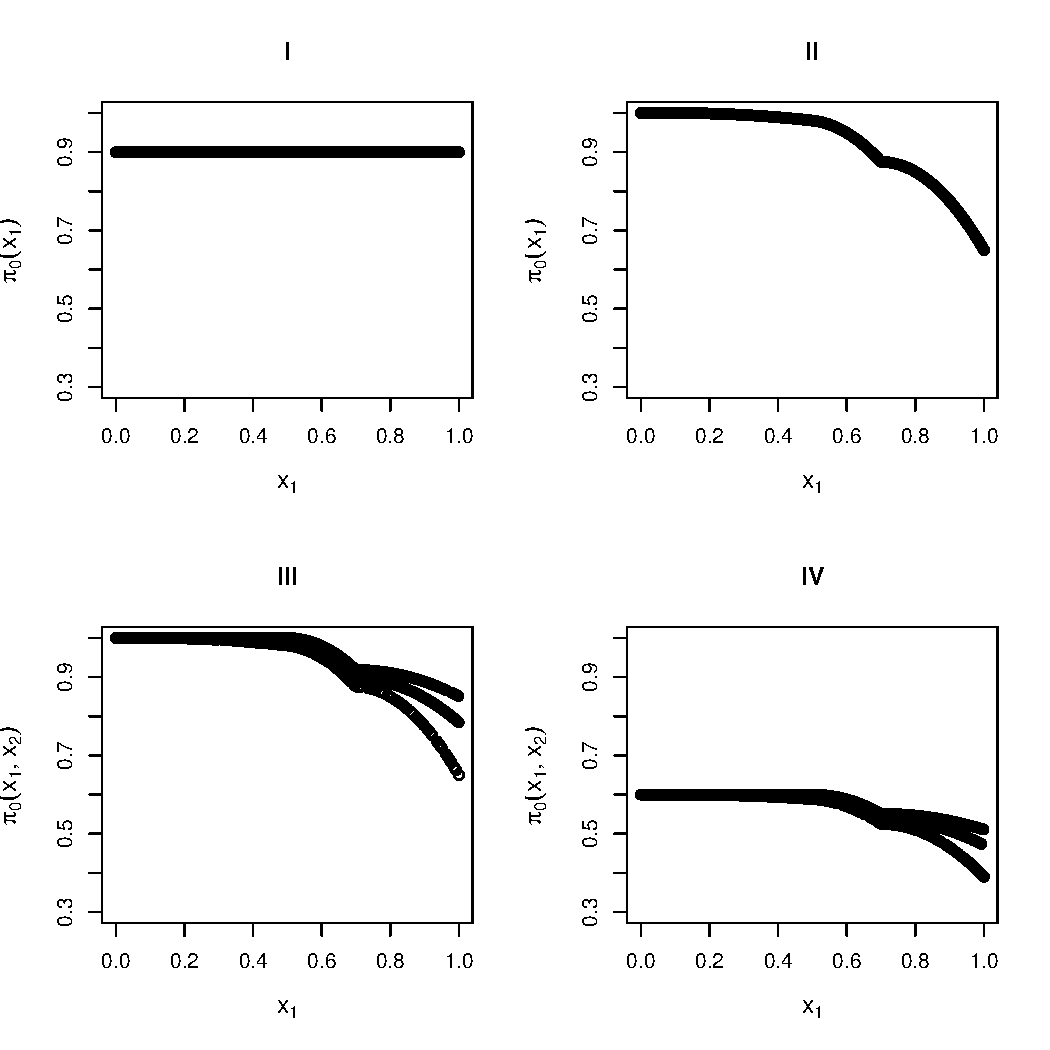
\includegraphics[width=\maxwidth]{Figures/Simulation_scenarios-1} 

}



\end{knitrout}

\noindent We performed 200 simulations in each scenario.
\\  
\noindent We estimated false discovery rates (FDR) and true positive rates (TPR) percentages for a nominal FDR of 5\%. 
We considered both the theoretical and empirical nulls for the Scott method.
For III and IV, a dummy variable was used for $x_{2}$, along with linear or spline terms (with 3 df) for $x_1$.

\clearpage

\subsection*{Independent test statistics}

We first generated independent test statistics.
\\
\noindent For the beta distribution, we generated the p-values directly from Beta(1,20). For the other distributions, we generated the test statistics and calculated the p-values from them.
For the t-test, we considered 2 groups of 6 (so 2x6 = 10 df) and used the t-statistics instead of the z-statistics for the Scott method. For the chisquared test, 1 df corresponds to a 2x2 table, 4 df to a 3x3 table. We used the z-statistics obtained from back-transforming the p-values for the Scott method for the beta and the chisquared cases.
\\
BL = Boca-Leek, Scott T = Scott theoretical null, Scott E = Scott empirical null

\subsubsection*{1,000 tests}





% latex table generated in R 3.3.1 by xtable 1.8-2 package
% Mon Jun 19 13:28:25 2017
\begin{table}[ht]
\centering
\begin{tabular}{lll|lllll|lllll}
  \hline
  &&& \multicolumn{5}{c}{FDR} & \multicolumn{5}{c}{TPR}\\
 $\pi_0(x)$ &  Dist. under $H_1$ & Reg. model & BL & Scott T & Scott E & Storey & BH & BL & Scott T & Scott E & Storey & BH    \\
 \hline
I & Beta(1,20) & Linear & 5.0 & 90.0 & 84.0 & 5.2 & 3.9 & 0.2 & 100.0 & 95.9 & 0.2 & 0.1 \\ 
  II & Beta(1,20) & Linear & 4.8 & 92.6 & 85.9 & 4.8 & 4.1 & 0.2 & 100.0 & 98.0 & 0.1 & 0.1 \\ 
  II & Beta(1,20) & Spline & 6.5 & 92.6 & 86.6 & 4.8 & 4.1 & 0.2 & 100.0 & 98.3 & 0.1 & 0.1 \\ 
  III & Beta(1,20) & Linear & 5.2 & 94.9 & 88.9 & 5.4 & 5.4 & 0.2 & 100.0 & 97.5 & 0.2 & 0.2 \\ 
  III & Beta(1,20) & Spline & 6.2 & 94.9 & 89.4 & 5.4 & 5.4 & 0.3 & 100.0 & 97.6 & 0.2 & 0.2 \\ 
  IV & Beta(1,20) & Linear & 6.4 & 56.7 &  & 5.1 & 3.4 & 12.2 & 100.0 &  & 5.4 & 0.3 \\ 
  IV & Beta(1,20) & Spline & 7.9 & 56.7 &  & 5.1 & 3.4 & 15.4 & 100.0 &  & 5.4 & 0.3 \\ 
   \hline
I & Norm & Linear & 5.0 & 5.2 & 6.6 & 4.9 & 4.4 & 51.0 & 50.9 & 49.7 & 50.8 & 49.7 \\ 
  II & Norm & Linear & 5.4 & 5.7 & 8.1 & 5.3 & 4.9 & 48.5 & 63.5 & 61.3 & 47.6 & 47.0 \\ 
  II & Norm & Spline & 5.6 & 5.9 & 8.3 & 5.3 & 4.9 & 49.3 & 63.5 & 61.5 & 47.6 & 47.0 \\ 
  III & Norm & Linear & 5.8 & 5.9 & 9.9 & 5.4 & 5.1 & 45.1 & 60.3 & 57.9 & 44.0 & 43.4 \\ 
  III & Norm & Spline & 5.9 & 6.0 & 10.1 & 5.4 & 5.1 & 45.6 & 60.9 & 58.2 & 44.0 & 43.4 \\ 
  IV & Norm & Linear & 5.0 & 4.9 & 2.4 & 4.7 & 2.8 & 71.6 & 71.8 & 60.6 & 71.2 & 65.4 \\ 
  IV & Norm & Spline & 5.2 & 5.0 & 2.4 & 4.7 & 2.8 & 72.0 & 71.9 & 60.7 & 71.2 & 65.4 \\ 
   \hline
I & T & Linear & 5.7 & 21.3 & 23.4 & 5.5 & 4.8 & 15.7 & 55.4 & 56.9 & 15.2 & 13.6 \\ 
  II & T & Linear & 4.8 & 20.7 & 23.8 & 5.0 & 4.4 & 13.0 & 64.5 & 65.5 & 11.6 & 10.6 \\ 
  II & T & Spline & 4.7 & 21.1 & 24.5 & 5.0 & 4.4 & 13.8 & 64.8 & 65.6 & 11.6 & 10.6 \\ 
  III & T & Linear & 6.2 & 26.8 & 31.0 & 5.9 & 5.4 & 9.4 & 54.6 & 54.7 & 8.2 & 7.6 \\ 
  III & T & Spline & 6.8 & 27.3 & 31.3 & 5.9 & 5.4 & 10.0 & 55.2 & 55.3 & 8.2 & 7.6 \\ 
  IV & T & Linear & 5.0 & 9.3 & 2.8 & 4.7 & 2.9 & 52.5 & 72.9 & 44.4 & 52.0 & 40.3 \\ 
  IV & T & Spline & 5.4 & 9.3 & 2.8 & 4.7 & 2.9 & 53.0 & 73.0 & 44.6 & 52.0 & 40.3 \\ 
   \hline
I & Chisq 1 df & Linear & 5.0 & 90.0 & 85.5 & 4.8 & 4.4 & 51.2 & 100.0 & 98.7 & 50.9 & 49.7 \\ 
  II & Chisq 1 df & Linear & 4.8 & 92.6 & 89.4 & 4.8 & 4.4 & 48.3 & 100.0 & 99.6 & 47.1 & 46.3 \\ 
  II & Chisq 1 df & Spline & 5.0 & 92.6 & 90.0 & 4.8 & 4.4 & 48.9 & 100.0 & 99.6 & 47.1 & 46.3 \\ 
  III & Chisq 1 df & Linear & 5.0 & 94.9 & 93.8 & 4.9 & 4.8 & 44.3 & 100.0 & 99.7 & 43.1 & 42.5 \\ 
  III & Chisq 1 df & Spline & 5.3 & 94.9 & 93.9 & 4.9 & 4.8 & 44.8 & 100.0 & 99.7 & 43.1 & 42.5 \\ 
  IV & Chisq 1 df & Linear & 5.1 & 56.7 &  & 4.7 & 2.8 & 71.6 & 100.0 &  & 71.1 & 65.1 \\ 
  IV & Chisq 1 df & Spline & 5.3 & 56.7 &  & 4.7 & 2.8 & 71.9 & 100.0 &  & 71.1 & 65.1 \\ 
   \hline
I & Chisq 4 df & Linear & 5.3 & 90.0 & 83.5 & 5.4 & 4.8 & 30.8 & 100.0 & 95.3 & 30.6 & 29.6 \\ 
  II & Chisq 4 df & Linear & 5.3 & 92.6 & 89.6 & 5.3 & 5.0 & 28.4 & 100.0 & 98.5 & 27.5 & 26.7 \\ 
  II & Chisq 4 df & Spline & 5.4 & 92.6 & 89.9 & 5.3 & 5.0 & 29.2 & 100.0 & 98.6 & 27.5 & 26.7 \\ 
  III & Chisq 4 df & Linear & 5.9 & 94.9 & 92.4 & 5.4 & 5.3 & 24.8 & 100.0 & 98.3 & 24.0 & 23.4 \\ 
  III & Chisq 4 df & Spline & 5.9 & 94.9 & 93.0 & 5.4 & 5.3 & 25.2 & 100.0 & 98.7 & 24.0 & 23.4 \\ 
  IV & Chisq 4 df & Linear & 5.1 & 56.7 & 55.9 & 4.7 & 2.8 & 52.3 & 100.0 & 98.8 & 51.7 & 44.5 \\ 
  IV & Chisq 4 df & Spline & 5.5 & 56.7 & 55.9 & 4.7 & 2.8 & 52.7 & 100.0 & 98.8 & 51.7 & 44.5 \\ 
   \hline
\end{tabular}
\end{table}


\clearpage

\subsubsection*{10,000 tests}





% latex table generated in R 3.3.1 by xtable 1.8-2 package
% Mon Jun 19 13:28:25 2017
\begin{table}[ht]
\centering
\begin{tabular}{lll|lllll|lllll}
  \hline
  &&& \multicolumn{5}{c}{FDR} & \multicolumn{5}{c}{TPR}\\
 $\pi_0(x)$ &  Dist. under $H_1$ & Reg. model & BL & Scott T & Scott E & Storey & BH & BL & Scott T & Scott E & Storey & BH    \\
 \hline
I & Beta(1,20) & Linear & 3.7 & 90.0 & 90.0 & 3.7 & 3.6 & 0.0 & 100.0 & 100.0 & 0.0 & 0.0 \\ 
  II & Beta(1,20) & Linear & 3.1 & 92.6 & 92.6 & 3.1 & 3.0 & 0.0 & 100.0 & 100.0 & 0.0 & 0.0 \\ 
  II & Beta(1,20) & Spline & 3.1 & 92.6 & 92.6 & 3.1 & 3.0 & 0.0 & 100.0 & 100.0 & 0.0 & 0.0 \\ 
  III & Beta(1,20) & Linear & 4.0 & 94.9 & 94.9 & 3.5 & 3.5 & 0.0 & 100.0 & 100.0 & 0.0 & 0.0 \\ 
  III & Beta(1,20) & Spline & 4.5 & 94.9 & 94.9 & 3.5 & 3.5 & 0.0 & 100.0 & 100.0 & 0.0 & 0.0 \\ 
  IV & Beta(1,20) & Linear & 4.4 & 56.9 &  & 4.8 & 2.5 & 1.2 & 100.0 &  & 0.5 & 0.0 \\ 
  IV & Beta(1,20) & Spline & 5.0 & 56.9 &  & 4.8 & 2.5 & 2.0 & 100.0 &  & 0.5 & 0.0 \\ 
   \hline
I & Norm & Linear & 5.0 & 5.0 & 5.9 & 5.0 & 4.5 & 50.6 & 50.6 & 52.1 & 50.7 & 49.6 \\ 
  II & Norm & Linear & 4.9 & 5.2 & 5.3 & 4.9 & 4.6 & 48.4 & 63.9 & 62.9 & 47.3 & 46.6 \\ 
  II & Norm & Spline & 4.9 & 5.2 & 5.3 & 4.9 & 4.6 & 48.8 & 64.0 & 63.0 & 47.3 & 46.6 \\ 
  III & Norm & Linear & 4.9 & 5.2 & 5.5 & 4.9 & 4.7 & 44.2 & 60.2 & 59.3 & 43.5 & 43.0 \\ 
  III & Norm & Spline & 4.9 & 5.2 & 5.4 & 4.9 & 4.7 & 44.4 & 60.6 & 59.7 & 43.5 & 43.0 \\ 
  IV & Norm & Linear & 4.8 & 5.0 & 2.3 & 4.8 & 2.8 & 71.3 & 71.8 & 62.2 & 71.2 & 65.3 \\ 
  IV & Norm & Spline & 4.8 & 5.0 & 2.3 & 4.8 & 2.8 & 71.3 & 71.8 & 62.2 & 71.2 & 65.3 \\ 
   \hline
I & T & Linear & 5.2 & 21.7 & 20.8 & 5.1 & 4.7 & 14.1 & 55.3 & 53.2 & 14.1 & 12.6 \\ 
  II & T & Linear & 4.6 & 20.0 & 19.9 & 4.9 & 4.5 & 11.5 & 65.7 & 65.4 & 10.2 & 9.2 \\ 
  II & T & Spline & 4.5 & 20.2 & 20.1 & 4.9 & 4.5 & 12.0 & 65.7 & 65.4 & 10.2 & 9.2 \\ 
  III & T & Linear & 4.9 & 24.7 & 26.8 & 5.2 & 5.2 & 6.8 & 62.5 & 63.7 & 6.0 & 5.5 \\ 
  III & T & Spline & 4.8 & 24.8 & 26.9 & 5.2 & 5.2 & 7.0 & 62.6 & 63.9 & 6.0 & 5.5 \\ 
  IV & T & Linear & 4.8 & 9.3 & 1.2 & 4.8 & 2.9 & 51.8 & 72.8 & 28.5 & 51.6 & 40.2 \\ 
  IV & T & Spline & 4.8 & 9.3 & 1.2 & 4.8 & 2.9 & 51.9 & 72.9 & 28.6 & 51.6 & 40.2 \\ 
   \hline
I & Chisq 1 df & Linear & 5.0 & 90.0 & 90.0 & 5.0 & 4.5 & 50.7 & 100.0 & 100.0 & 50.6 & 49.6 \\ 
  II & Chisq 1 df & Linear & 4.9 & 92.6 & 92.6 & 5.0 & 4.6 & 48.2 & 100.0 & 100.0 & 47.2 & 46.4 \\ 
  II & Chisq 1 df & Spline & 4.8 & 92.6 & 92.6 & 5.0 & 4.6 & 48.6 & 100.0 & 100.0 & 47.2 & 46.4 \\ 
  III & Chisq 1 df & Linear & 5.0 & 94.9 & 94.9 & 5.0 & 4.8 & 44.0 & 100.0 & 100.0 & 43.2 & 42.7 \\ 
  III & Chisq 1 df & Spline & 5.0 & 94.9 & 94.9 & 5.0 & 4.8 & 44.2 & 100.0 & 100.0 & 43.2 & 42.7 \\ 
  IV & Chisq 1 df & Linear & 4.8 & 56.9 &  & 4.8 & 2.8 & 71.1 & 100.0 &  & 71.0 & 65.2 \\ 
  IV & Chisq 1 df & Spline & 4.8 & 56.9 &  & 4.8 & 2.8 & 71.2 & 100.0 &  & 71.0 & 65.2 \\ 
   \hline
I & Chisq 4 df & Linear & 5.0 & 90.0 & 90.0 & 5.0 & 4.5 & 29.7 & 100.0 & 100.0 & 29.7 & 28.7 \\ 
  II & Chisq 4 df & Linear & 4.9 & 92.6 & 92.6 & 5.0 & 4.7 & 28.0 & 100.0 & 100.0 & 27.1 & 26.5 \\ 
  II & Chisq 4 df & Spline & 4.9 & 92.6 & 92.6 & 5.0 & 4.7 & 28.4 & 100.0 & 100.0 & 27.1 & 26.5 \\ 
  III & Chisq 4 df & Linear & 5.2 & 94.9 & 94.9 & 5.2 & 5.0 & 24.3 & 100.0 & 100.0 & 23.6 & 23.2 \\ 
  III & Chisq 4 df & Spline & 5.2 & 94.9 & 94.9 & 5.2 & 5.0 & 24.4 & 100.0 & 100.0 & 23.6 & 23.2 \\ 
  IV & Chisq 4 df & Linear & 4.7 & 56.9 & 57.1 & 4.7 & 2.8 & 51.8 & 100.0 & 100.0 & 51.7 & 44.8 \\ 
  IV & Chisq 4 df & Spline & 4.7 & 56.9 & 57.1 & 4.7 & 2.8 & 51.9 & 100.0 & 100.0 & 51.7 & 44.8 \\ 
   \hline
\end{tabular}
\end{table}


\clearpage

\subsection*{Dependent test statistics - 1,000 tests}

We next generated independent test statistics. We used multivariate normal and t distributions (10 df for the t-distribution). 
We considered block-diagnonal matrices with the number of blocks equal to 20 or 10 and the within-block correlation, $\rho$, of 0.2, 0.5, or 0.9. Thus, 20 blocks meant a block size of 50 tests (lesser dependence) and 10 blocks a block size of 100 tests (more dependence).
\\
BL = Boca-Leek, Scott T = Scott theoretical null, Scott E = Scott empirical null




  
% latex table generated in R 3.3.1 by xtable 1.8-2 package
% Mon Jun 19 13:28:25 2017
\begin{table}[ht]
\centering
\begin{tabular}{lll|lllll|lllll}
  \hline
  &&& \multicolumn{5}{c}{FDR} & \multicolumn{5}{c}{TPR}\\
 $\pi_0(x)$ &  Dist. under $H_1$ & Reg. model & BL & Scott T & Scott E & Storey & BH & BL & Scott T & Scott E & Storey & BH    \\
 \hline
I & N, 20 blocks, $\rho$=0.2 & Linear & 5.3 & 6.2 & 6.8 & 5.0 & 4.4 & 51.5 & 51.4 & 48.4 & 51.3 & 50.1 \\ 
  II & N, 20 blocks, $\rho$=0.2 & Linear & 5.2 & 6.9 & 8.0 & 5.1 & 4.6 & 48.6 & 63.4 & 59.3 & 47.6 & 46.5 \\ 
  II & N, 20 blocks, $\rho$=0.2 & Spline & 5.7 & 8.3 & 9.2 & 5.1 & 4.6 & 49.2 & 63.3 & 59.6 & 47.6 & 46.5 \\ 
  III & N, 20 blocks, $\rho$=0.2 & Linear & 5.5 & 7.6 & 9.3 & 5.2 & 4.8 & 45.1 & 60.0 & 56.0 & 44.0 & 43.2 \\ 
  III & N, 20 blocks, $\rho$=0.2 & Spline & 5.7 & 9.6 & 10.6 & 5.2 & 4.8 & 45.9 & 60.2 & 56.3 & 44.0 & 43.2 \\ 
  IV & N, 20 blocks, $\rho$=0.2 & Linear & 5.3 & 5.3 & 2.5 & 4.9 & 2.9 & 71.8 & 71.9 & 61.0 & 71.4 & 65.6 \\ 
  IV & N, 20 blocks, $\rho$=0.2 & Spline & 5.6 & 5.5 & 2.5 & 4.9 & 2.9 & 72.0 & 71.9 & 61.1 & 71.4 & 65.6 \\ 
   \hline
I & N, 20 blocks, $\rho$=0.5 & Linear & 6.4 & 10.0 & 10.7 & 6.0 & 5.2 & 52.0 & 51.7 & 47.6 & 51.6 & 50.3 \\ 
  II & N, 20 blocks, $\rho$=0.5 & Linear & 6.1 & 12.4 & 13.5 & 5.7 & 5.1 & 48.4 & 62.8 & 57.6 & 47.3 & 46.2 \\ 
  II & N, 20 blocks, $\rho$=0.5 & Spline & 7.1 & 18.7 & 20.4 & 5.7 & 5.1 & 49.5 & 62.6 & 58.0 & 47.3 & 46.2 \\ 
  III & N, 20 blocks, $\rho$=0.5 & Linear & 5.6 & 11.5 & 15.9 & 5.2 & 4.6 & 45.4 & 59.6 & 56.6 & 44.0 & 43.2 \\ 
  III & N, 20 blocks, $\rho$=0.5 & Spline & 6.6 & 19.9 & 23.6 & 5.2 & 4.6 & 46.2 & 59.0 & 56.9 & 44.0 & 43.2 \\ 
  IV & N, 20 blocks, $\rho$=0.5 & Linear & 5.8 & 6.1 & 2.8 & 5.3 & 3.1 & 72.1 & 72.3 & 59.4 & 71.6 & 65.7 \\ 
  IV & N, 20 blocks, $\rho$=0.5 & Spline & 6.5 & 6.4 & 3.0 & 5.3 & 3.1 & 72.4 & 72.2 & 59.6 & 71.6 & 65.7 \\ 
   \hline
I & N, 20 blocks, $\rho$=0.9 & Linear & 9.0 & 17.6 & 36.2 & 6.9 & 5.3 & 53.8 & 53.3 & 57.9 & 52.6 & 50.4 \\ 
  II & N, 20 blocks, $\rho$=0.9 & Linear & 7.8 & 20.0 & 47.5 & 6.4 & 4.9 & 49.6 & 63.8 & 68.0 & 48.0 & 46.2 \\ 
  II & N, 20 blocks, $\rho$=0.9 & Spline & 18.2 & 34.5 & 53.6 & 6.4 & 4.9 & 52.2 & 64.4 & 69.8 & 48.0 & 46.2 \\ 
  III & N, 20 blocks, $\rho$=0.9 & Linear & 6.4 & 23.1 & 48.8 & 5.1 & 4.0 & 47.3 & 60.5 & 67.9 & 46.1 & 44.0 \\ 
  III & N, 20 blocks, $\rho$=0.9 & Spline & 21.5 & 38.4 & 60.5 & 5.1 & 4.0 & 51.0 & 60.9 & 69.7 & 46.1 & 44.0 \\ 
  IV & N, 20 blocks, $\rho$=0.9 & Linear & 7.7 & 8.4 & 6.9 & 6.1 & 3.1 & 73.1 & 73.2 & 57.4 & 72.2 & 65.9 \\ 
  IV & N, 20 blocks, $\rho$=0.9 & Spline & 11.8 & 10.0 & 8.0 & 6.1 & 3.1 & 74.4 & 72.8 & 57.8 & 72.2 & 65.9 \\ 
   \hline
I & N, 10 blocks, $\rho$=0.2 & Linear & 5.4 & 7.8 & 6.1 & 5.1 & 4.4 & 51.6 & 51.6 & 47.3 & 51.2 & 49.9 \\ 
  II & N, 10 blocks, $\rho$=0.2 & Linear & 5.0 & 9.3 & 8.8 & 4.8 & 4.3 & 48.2 & 63.0 & 59.8 & 47.2 & 46.1 \\ 
  II & N, 10 blocks, $\rho$=0.2 & Spline & 5.5 & 13.3 & 11.1 & 4.8 & 4.3 & 49.1 & 62.8 & 59.8 & 47.2 & 46.1 \\ 
  III & N, 10 blocks, $\rho$=0.2 & Linear & 5.2 & 8.6 & 9.8 & 5.0 & 4.5 & 44.6 & 59.5 & 56.4 & 43.4 & 42.7 \\ 
  III & N, 10 blocks, $\rho$=0.2 & Spline & 5.8 & 14.3 & 13.2 & 5.0 & 4.5 & 45.2 & 59.2 & 56.6 & 43.4 & 42.7 \\ 
  IV & N, 10 blocks, $\rho$=0.2 & Linear & 5.3 & 5.7 & 2.4 & 5.0 & 2.9 & 71.8 & 71.8 & 60.4 & 71.4 & 65.5 \\ 
  IV & N, 10 blocks, $\rho$=0.2 & Spline & 5.7 & 5.9 & 2.5 & 5.0 & 2.9 & 72.1 & 71.8 & 60.5 & 71.4 & 65.5 \\ 
   \hline
I & N, 10 blocks, $\rho$=0.5 & Linear & 7.3 & 17.1 & 15.9 & 6.5 & 5.4 & 51.9 & 51.8 & 48.8 & 51.7 & 50.0 \\ 
  II & N, 10 blocks, $\rho$=0.5 & Linear & 5.9 & 20.3 & 19.9 & 5.3 & 4.5 & 48.3 & 62.6 & 61.0 & 46.8 & 45.6 \\ 
  II & N, 10 blocks, $\rho$=0.5 & Spline & 8.6 & 32.5 & 27.7 & 5.3 & 4.5 & 49.2 & 63.3 & 61.4 & 46.8 & 45.6 \\ 
  III & N, 10 blocks, $\rho$=0.5 & Linear & 5.8 & 17.4 & 17.7 & 4.9 & 4.2 & 44.2 & 58.1 & 54.3 & 43.0 & 42.0 \\ 
  III & N, 10 blocks, $\rho$=0.5 & Spline & 8.6 & 32.7 & 30.2 & 4.9 & 4.2 & 45.0 & 58.1 & 55.6 & 43.0 & 42.0 \\ 
  IV & N, 10 blocks, $\rho$=0.5 & Linear & 6.3 & 7.5 & 3.3 & 5.5 & 3.2 & 72.4 & 72.4 & 59.0 & 71.9 & 65.8 \\ 
  IV & N, 10 blocks, $\rho$=0.5 & Spline & 7.6 & 8.3 & 3.8 & 5.5 & 3.2 & 72.7 & 72.1 & 59.3 & 71.9 & 65.8 \\ 
   \hline
I & N, 10 blocks, $\rho$=0.9 & Linear & 14.1 & 30.6 & 45.6 & 6.6 & 4.1 & 55.5 & 54.7 & 65.6 & 53.3 & 50.2 \\ 
  II & N, 10 blocks, $\rho$=0.9 & Linear & 13.3 & 35.5 & 55.9 & 5.9 & 3.3 & 51.1 & 66.5 & 75.8 & 49.0 & 46.1 \\ 
  II & N, 10 blocks, $\rho$=0.9 & Spline & 35.1 & 49.9 & 67.5 & 5.9 & 3.3 & 56.1 & 67.4 & 77.6 & 49.0 & 46.1 \\ 
  III & N, 10 blocks, $\rho$=0.9 & Linear & 13.3 & 33.7 & 66.4 & 5.4 & 3.3 & 45.6 & 58.1 & 75.7 & 43.4 & 40.7 \\ 
  III & N, 10 blocks, $\rho$=0.9 & Spline & 40.7 & 51.5 & 73.0 & 5.4 & 3.3 & 52.0 & 61.6 & 77.4 & 43.4 & 40.7 \\ 
  IV & N, 10 blocks, $\rho$=0.9 & Linear & 11.2 & 12.4 & 12.0 & 7.0 & 3.1 & 74.0 & 73.5 & 63.9 & 72.5 & 65.8 \\ 
  IV & N, 10 blocks, $\rho$=0.9 & Spline & 19.2 & 15.6 & 13.8 & 7.0 & 3.1 & 76.2 & 73.3 & 64.3 & 72.5 & 65.8 \\ 
   \hline
\end{tabular}
\end{table}


% latex table generated in R 3.3.1 by xtable 1.8-2 package
% Mon Jun 19 13:28:25 2017
\begin{table}[ht]
\centering
\begin{tabular}{lll|lllll|lllll}
  \hline
  &&& \multicolumn{5}{c}{FDR} & \multicolumn{5}{c}{TPR}\\
 $\pi_0(x)$ &  Dist. under $H_1$ & Reg. model & BL & Scott T & Scott E & Storey & BH & BL & Scott T & Scott E & Storey & BH    \\
 \hline
I & T, 20 blocks, $\rho$=0.2 & Linear & 1.7 & 9.1 & 7.4 & 1.5 & 0.9 & 8.0 & 51.6 & 57.8 & 7.6 & 5.7 \\ 
  II & T, 20 blocks, $\rho$=0.2 & Linear & 3.2 & 13.9 & 7.3 & 3.2 & 1.8 & 8.0 & 63.8 & 61.0 & 6.8 & 4.5 \\ 
  II & T, 20 blocks, $\rho$=0.2 & Spline & 3.7 & 14.7 & 8.5 & 3.2 & 1.8 & 9.2 & 63.9 & 61.3 & 6.8 & 4.5 \\ 
  III & T, 20 blocks, $\rho$=0.2 & Linear & 2.6 & 13.8 & 9.6 & 2.1 & 1.3 & 4.3 & 59.4 & 60.1 & 3.4 & 2.3 \\ 
  III & T, 20 blocks, $\rho$=0.2 & Spline & 3.6 & 15.1 & 11.0 & 2.1 & 1.3 & 5.2 & 59.7 & 60.3 & 3.4 & 2.3 \\ 
  IV & T, 20 blocks, $\rho$=0.2 & Linear & 2.7 & 5.4 & 2.9 & 2.4 & 1.0 & 55.4 & 71.8 & 65.1 & 54.4 & 44.3 \\ 
  IV & T, 20 blocks, $\rho$=0.2 & Spline & 3.0 & 5.4 & 2.8 & 2.4 & 1.0 & 56.0 & 71.9 & 65.1 & 54.4 & 44.3 \\ 
   \hline
I & T, 20 blocks, $\rho$=0.5 & Linear & 1.7 & 10.3 & 11.0 & 1.5 & 1.0 & 8.6 & 51.6 & 57.4 & 8.2 & 5.9 \\ 
  II & T, 20 blocks, $\rho$=0.5 & Linear & 3.5 & 16.3 & 11.9 & 3.3 & 2.1 & 7.7 & 64.2 & 61.7 & 6.6 & 4.5 \\ 
  II & T, 20 blocks, $\rho$=0.5 & Spline & 4.7 & 19.5 & 16.6 & 3.3 & 2.1 & 9.1 & 63.9 & 62.1 & 6.6 & 4.5 \\ 
  III & T, 20 blocks, $\rho$=0.5 & Linear & 3.2 & 17.6 & 13.0 & 2.3 & 1.5 & 5.0 & 59.3 & 59.0 & 3.6 & 2.6 \\ 
  III & T, 20 blocks, $\rho$=0.5 & Spline & 4.4 & 23.4 & 20.5 & 2.3 & 1.5 & 5.6 & 59.6 & 59.5 & 3.6 & 2.6 \\ 
  IV & T, 20 blocks, $\rho$=0.5 & Linear & 2.7 & 5.5 & 3.0 & 2.3 & 1.0 & 55.3 & 71.9 & 64.7 & 54.3 & 44.4 \\ 
  IV & T, 20 blocks, $\rho$=0.5 & Spline & 3.2 & 5.8 & 3.1 & 2.3 & 1.0 & 55.8 & 71.9 & 64.8 & 54.3 & 44.4 \\ 
   \hline
I & T, 20 blocks, $\rho$=0.9 & Linear & 3.0 & 14.5 & 29.0 & 1.5 & 0.9 & 11.5 & 51.7 & 64.1 & 9.9 & 6.2 \\ 
  II & T, 20 blocks, $\rho$=0.9 & Linear & 3.8 & 20.9 & 45.7 & 2.3 & 1.9 & 10.2 & 64.9 & 70.6 & 7.7 & 5.0 \\ 
  II & T, 20 blocks, $\rho$=0.9 & Spline & 15.8 & 32.1 & 54.6 & 2.3 & 1.9 & 14.2 & 64.7 & 70.5 & 7.7 & 5.0 \\ 
  III & T, 20 blocks, $\rho$=0.9 & Linear & 5.2 & 23.9 & 49.7 & 3.2 & 1.4 & 7.3 & 60.7 & 63.5 & 5.6 & 3.1 \\ 
  III & T, 20 blocks, $\rho$=0.9 & Spline & 19.0 & 35.1 & 60.6 & 3.2 & 1.4 & 10.6 & 61.7 & 65.5 & 5.6 & 3.1 \\ 
  IV & T, 20 blocks, $\rho$=0.9 & Linear & 3.6 & 6.6 & 7.5 & 2.4 & 1.0 & 56.1 & 72.2 & 67.5 & 54.6 & 44.3 \\ 
  IV & T, 20 blocks, $\rho$=0.9 & Spline & 8.6 & 7.5 & 8.0 & 2.4 & 1.0 & 58.4 & 72.0 & 67.2 & 54.6 & 44.3 \\ 
   \hline
I & T, 10 blocks, $\rho$=0.2 & Linear & 1.8 & 9.9 & 7.8 & 1.6 & 0.8 & 8.3 & 51.3 & 57.2 & 8.0 & 5.9 \\ 
  II & T, 10 blocks, $\rho$=0.2 & Linear & 3.4 & 15.0 & 8.1 & 3.4 & 1.5 & 7.3 & 63.1 & 61.3 & 6.4 & 4.3 \\ 
  II & T, 10 blocks, $\rho$=0.2 & Spline & 4.0 & 16.7 & 9.9 & 3.4 & 1.5 & 8.6 & 63.2 & 61.5 & 6.4 & 4.3 \\ 
  III & T, 10 blocks, $\rho$=0.2 & Linear & 2.2 & 15.2 & 9.5 & 1.6 & 1.2 & 3.7 & 58.7 & 59.4 & 3.0 & 1.9 \\ 
  III & T, 10 blocks, $\rho$=0.2 & Spline & 2.7 & 18.0 & 12.7 & 1.6 & 1.2 & 4.2 & 58.5 & 59.7 & 3.0 & 1.9 \\ 
  IV & T, 10 blocks, $\rho$=0.2 & Linear & 2.6 & 5.5 & 2.8 & 2.4 & 1.0 & 54.8 & 71.5 & 64.6 & 53.9 & 43.9 \\ 
  IV & T, 10 blocks, $\rho$=0.2 & Spline & 3.0 & 5.6 & 2.8 & 2.4 & 1.0 & 55.4 & 71.5 & 64.7 & 53.9 & 43.9 \\ 
   \hline
I & T, 10 blocks, $\rho$=0.5 & Linear & 2.2 & 13.5 & 14.2 & 1.6 & 0.9 & 9.3 & 50.8 & 57.4 & 8.5 & 6.1 \\ 
  II & T, 10 blocks, $\rho$=0.5 & Linear & 3.3 & 19.2 & 13.6 & 3.4 & 1.7 & 7.9 & 63.1 & 61.2 & 7.0 & 4.4 \\ 
  II & T, 10 blocks, $\rho$=0.5 & Spline & 6.2 & 27.6 & 21.3 & 3.4 & 1.7 & 9.9 & 63.5 & 61.3 & 7.0 & 4.4 \\ 
  III & T, 10 blocks, $\rho$=0.5 & Linear & 2.3 & 23.4 & 21.5 & 1.3 & 0.7 & 4.4 & 58.0 & 59.5 & 3.0 & 2.1 \\ 
  III & T, 10 blocks, $\rho$=0.5 & Spline & 3.8 & 35.9 & 31.4 & 1.3 & 0.7 & 5.6 & 58.1 & 60.1 & 3.0 & 2.1 \\ 
  IV & T, 10 blocks, $\rho$=0.5 & Linear & 3.1 & 6.1 & 3.4 & 2.5 & 1.0 & 54.4 & 71.4 & 63.5 & 53.4 & 43.2 \\ 
  IV & T, 10 blocks, $\rho$=0.5 & Spline & 4.3 & 6.6 & 3.8 & 2.5 & 1.0 & 55.3 & 71.2 & 64.0 & 53.4 & 43.2 \\ 
   \hline
I & T, 10 blocks, $\rho$=0.9 & Linear & 7.7 & 23.0 & 38.0 & 1.6 & 1.0 & 14.9 & 51.5 & 70.9 & 11.4 & 6.7 \\ 
  II & T, 10 blocks, $\rho$=0.9 & Linear & 10.1 & 31.5 & 50.0 & 4.1 & 1.7 & 12.4 & 65.4 & 76.2 & 11.1 & 6.0 \\ 
  II & T, 10 blocks, $\rho$=0.9 & Spline & 41.7 & 43.6 & 60.7 & 4.1 & 1.7 & 22.4 & 68.2 & 78.9 & 11.1 & 6.0 \\ 
  III & T, 10 blocks, $\rho$=0.9 & Linear & 12.7 & 36.2 & 62.9 & 2.2 & 1.3 & 11.0 & 60.5 & 77.2 & 5.8 & 2.6 \\ 
  III & T, 10 blocks, $\rho$=0.9 & Spline & 43.0 & 48.4 & 71.0 & 2.2 & 1.3 & 19.3 & 62.9 & 78.7 & 5.8 & 2.6 \\ 
  IV & T, 10 blocks, $\rho$=0.9 & Linear & 6.2 & 9.2 & 11.1 & 3.2 & 1.0 & 56.3 & 72.1 & 68.3 & 54.2 & 42.4 \\ 
  IV & T, 10 blocks, $\rho$=0.9 & Spline & 15.1 & 10.8 & 11.8 & 3.2 & 1.0 & 59.3 & 71.8 & 68.3 & 54.2 & 42.4 \\ 
   \hline
\end{tabular}
\end{table}



\end{document}
